% ***************************************
% ***************************************
\chapter{Background} \label{background}
% ***************************************
% ***************************************
In this chapter the background knowledge useful to understand this thesis is described as well as the previous work done by other scientist in the area to give an overview of what has been done previously and how this research advances it. The first section will describe the basics of Genomics applied to LOAD, as well as the main tools and procedures used to generate, process and evaluate the dataset. Afterwards, a more in-depth description of Alzheimer's disease and the factors that make it up and possible causes is given.  The next section will describe the basics of Machine Learning as well as the methods used in this thesis: Support Vector Machines, Random Forest, Neural Networks and Deep Networks, and the FRESA.CAD Benchmark.  Finally, the research done with Machine Learning for the prediction of genetic diseases, the detection of Alzheimer's and the prediction of Alzheimer's is shown.

\section{Genomics}

Genomics is the study of the genome of individuals or species. The genome encodes the genetic information across different chromosomes, which in turn can be divided in functional units of genes made up of a varying number of base pairs. These base pairs are the building blocks of the entire genome, and a single mutation can have a strong enough impact which substantially alters the health of an individual. Multiple ways exist to analyze genomics data and as more data is available when the use of sequencing is more widespread the clinical possibilities of finding (And hopefully treating) the genetic variations linked to diseases will greatly increase.
\newpage
This section gives the background information of genetics used in this thesis. The first section give a brief introduction to genetic variants, polymorphisms and Genome sequencing. The next section describes the Linkage Disequilibrium and Missing Heritability problem. Afterwards a primer on Genome-Wise Association studies (GWAS) is given and their use for genetic diseases. Next, Polygenic Risk Scores (PRS) are characterized and how they relate to GWAS. Complementing this, the PRS-based LDPred-funct method is described further.

 
\subsection{Genetic Variation, Polymorphisms and Sequencing}

Human variation is an interesting occurrence. 95\% of the human genome is shared across all of the humans. But that ~5\% is enough to provide all the variation we can see all around us every day. There are approximately 90 million of SNPs detected with at least 1 variation and that percentage is informative enough to find phenotypes (The physiological expression of a genotype) that might be of interest clinically. Additionally, the scale and complexity of the Human Genome presents a series of challenges, with over 3 billion nucleotides and multiple mechanisms that modify it.\cite{nussbaum_mcinnes_willard_2016}

Because of the huge variance between different populations and the distinct interactions particular to each population a comparison should almost always be handled within the same population. A gene variant in one population could have no effect and with another population have a greater impact. Plus, statistically the allele frequencies vary too much to be able to compare them usefully.\cite{nussbaum_mcinnes_willard_2016}

Different types of mutations occur in the genome, ranging from chromosomal mutations that affect an entire chromosome, to mutations that modify a segment of the chromosome, and mutations that substitute, insert or delete sequences of DNA at a given position of the genome(named as locus).\cite{nussbaum_mcinnes_willard_2016}


The main unit of reference in the genome is the locus, which is a given location in the genome and could be a single nucleotide or a group of genes. In a given locus there can be different possible variants of the DNA sequence which are named alleles. There tends to be a statistically common variant of the allele which is considered the reference allele, and alternate variant alleles that commonly arise from genetic mutation. Furthermore, these allele variants can be classified in two classes: those which occur in more than 1\% of the population are common enough to be called as having a polymorphism, and those with a frequency lower which are traditionally known as rare variants.\cite{nussbaum_mcinnes_willard_2016}
\newpage
The simplest, most common, most studied and useful mutation are Single-nucleotide Polymorphism. These are mutations where a a single locus has just two possible alleles that consist of a single substitution in a base, as shown in Figure \ref{genfig2}. SNPs can occur in non-coding regions, in introns and regions far from known genes, but this won't be delved into, as most SNPs that affect health are those that occur in protein-coding sequences which end up modifying the structure of the protein causing a biochemical impact. Most of the known genetic diseases are caused by these SNP and as such will be the focus of the thesis.\cite{nussbaum_mcinnes_willard_2016}

\begin{figure}[!ht]
\centerline{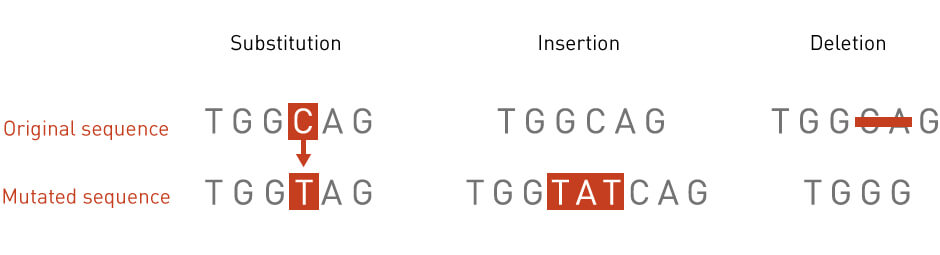
\includegraphics[width=4in]{images/background/muts.jpg}}
\caption{{\bf Some types of nucleotide mutations\cite{muts}} This shows the three most common variations. The SNP is on the left, then an insertion where a sequence is inserted, and the deletion where the opposite occurs}
\label{genfig2}
\end{figure}

Some diseases such as cystic fibrosis or sickle-cell anemia are inherited by a single gene that has mutated. These traits or diseases are called Mendelian because they follow a classical model of inheritance pattern which Mendel first described. Contrary to what may appear Mendelian diseases can happen with different variations in the same gene, with the same variation in the same gene, or with mutations in different genes that end up causing the same phenotype. All of these though are characterized by being caused by just one mutation. Predicting these types of diseases (or the risk of transmitting the disease to offspring) is easy to do, as just specific markers need to be analyzed and contrasted against common variants.\cite{nussbaum_mcinnes_willard_2016}
\newpage
In contrast, there are some diseases which are multifactorial and have a complex inheritance, such as Alzheimer's Disease, neuropsychiatric disorders or heart diseases. These diseases do not follow a Mendelian pattern of inheritance, and instead are thought to arise from complex interactions across different genes which modify the susceptibility to the given disease, and are then also affected by environmental factors as well as luck factors. Predicting these diseases is much more complicated and requires a broader set of factors to obtain meaningful results.\cite{nussbaum_mcinnes_willard_2016}

Knowledge about these mutations is only useful if the individual has a way of "reading" their DNA. This is done using Genome Sequencing, which allows analyzing sequences of base pairs to obtaining the existing DNA code in cells. Genome sequencing used to be prohibitively expensive 20 years ago but has since become much more affordable such that the general public can now use it (the first genome costed 2.7 billion USD , while it can now be obtained for 100-1000 USD). There are different types of Genome Sequencing: Whole-Genome Sequencing (WES)and Whole-Exome Sequencing (WES). The difference between the two is just a matter of scope, the second only analyzes the Exome, which is the 2\% of the genome containing exons (The protein-coding DNA). Generally WGS studies tend to have much more variants and information than WES, although the second ones are cheaper and thus could be used if the relationships are found in the exome. The specifics of the implementation of each won't be delved upon.



\subsection{Linkage (Dis)Equilibrium and Missing Heritability}
\label{missHerit}
One of the most important features of genetic analysis is Linkage. Linkage refers to the fact that due to natural selection, mutation, genetic drift and other biological and historical causes some alleles from different loci (and nearby in the genome) are associated in a non-random manner at a population level(That is, they are generally inherited together). Alleles are in Linkage Equilibrium when each Allele is independent of each other, conversely if they appear together with similar frequencies they are in Disequilibrium (LD), one such example analysis can be seen in figure \ref{genfig3}.\cite{nussbaum_mcinnes_willard_2016}

\begin{figure}[!ht]
\centerline{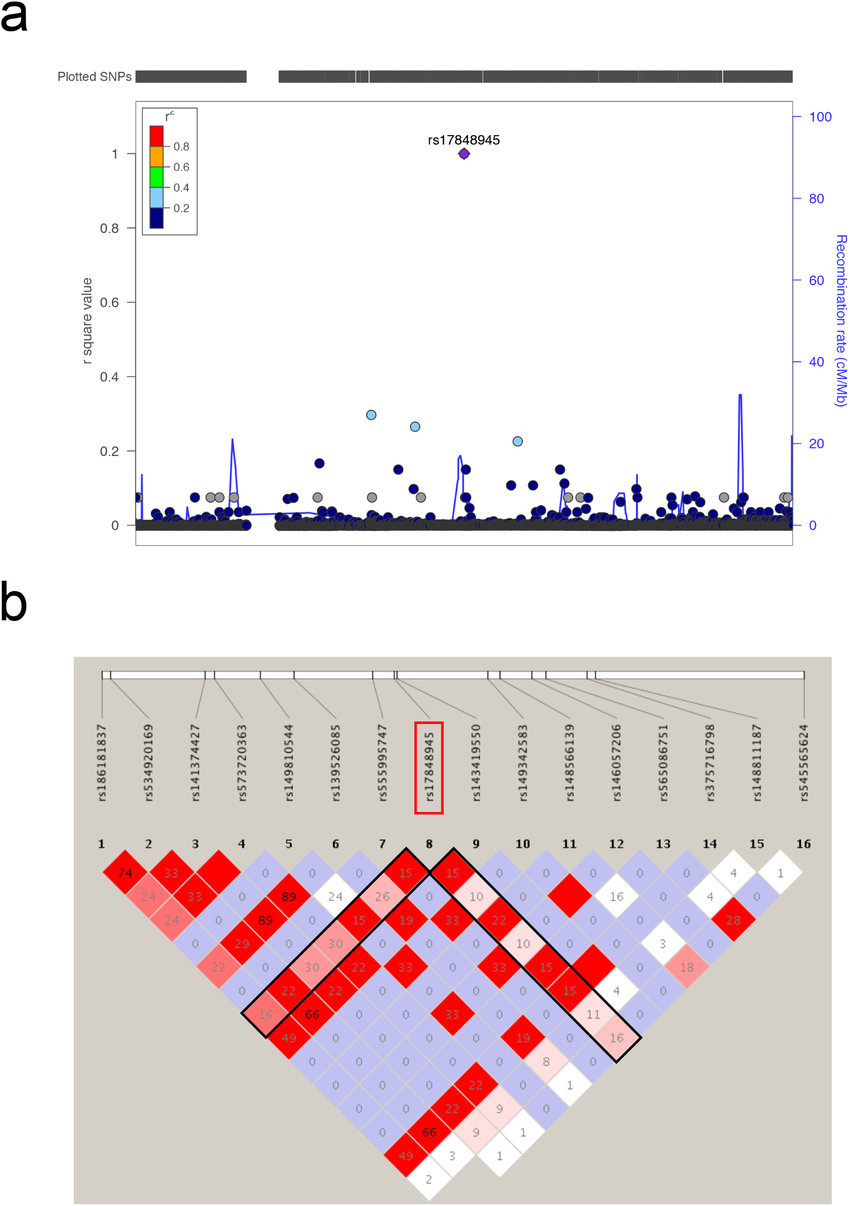
\includegraphics[width=4in,height=5in]{images/background/ld.jpg}}
\caption{{\bf Example of LD plots of marker rs17848945 \cite{ldfig}} Image a) gives the LD plot of the given SNP and the $R^2$ value of close SNPs. Image b) shows the LD block plot for further correlation analysis}
\label{genfig3}
\end{figure}

This has both positive and negative consequences. Positive, because if two alleles are closely linked, one can know the existence of one of those allele by proxy when knowing the other allele. This is useful for some tools such as Genome-Wide Association Studies and to do Linkage Analysis for detecting familiar diseases. Negative, because for predictive models this association between gene variants means that the system is fed inputs which are in correlation with each other and could generate results that are not valid or consistent, thus multiple those genes in linkage need to be processed in a way that they do not affect the data.\cite{nussbaum_mcinnes_willard_2016}

Another issue that complicates matters regarding genetic analysis is the Missing Heritability problem. One way to measure the genetic Heritability of a disease is with the use of Twin Studies, where genetic twins sharing the same genetic material are studied across different families to see if the disease or trait is genetic in nature or if it is environmental ( or a combination of both). Using these studies there are many multiple diseases which have been shown to have a medium-high genetic component, but when doing genetic studies the heritability that single SNPs or a mix of few foreground genes can explain is nowhere close to the estimated values of twin studies. Thus the genetic variations are unable to sufficiently explain the genetic factor estimated. One plausible theory is that the genetic influence is spread out across a multitude of background genes and interactions between them, instead of being an additive risk. Other theories discuss epigenetics, non-coding and exotic variants. As larger and more complete studies are done the highly polygenic hypothesis can be ascertained and validates.

\subsection{Genome-Wide Association Study}
\label{GWAS}
Genome-Wide Association Studies are one way to detect which gene variants are responsible or directly linked to a given disease by analyzing the whole genome in an statistical manner using a very large number of samples. They typically map the genome using millions of variants, taking advantage of the Linkage Disequilibrium phenomena. This is because if they map a variant which is in LD with the real variant related to the disease this correlation will then be visible in the variant mapped. In such a way, by using markers slightly spaced out they can reliably map the expected interaction of almost the entire genome with a fraction of the cost. And by obtaining samples from a very large group the statistical correlation between phenotype and the linked variants will appear (if it exists) thanks to the sample size.\cite{nussbaum_mcinnes_willard_2016}


One risk of GWAS though is population stratification, if subgroups exist within the data set the statistical results could find regional variants to be linked to the disease, thus care must be taken to ensure the population is the same for all samples. Another possible detail required is to limit the significance values strictly, as having such a big number of possible variants there is a high probability that by pure luck one out of the million SNPs will be close enough to be marked as significant when it is not. GWAS give an indication of the statistical relationship existing between a variant and a disease, with this a biochemical reason can be looked for in the candidate biomarkers to ensure the relationship is not purely statistical. Additionally, GWAS have shown proof than multiple common diseases are genetically complex in nature as well as highly polygenic.\cite{nussbaum_mcinnes_willard_2016}

\clearpage
\subsection{Polygenic Risk Scores}
\label{PRS}
As shown in previous subsections, the underlying hypothesis is that many complex diseases are characterized by being highly polygenic in nature, with each variant giving a very small adjustment in the risk, but when added up or combined together in a non-additive manner the genetic explanation starts to become much more robust and can explain a higher percentage of the missing heritability.

Extending this idea, Polygenic Risk Scores(PRS)\cite{pers} come as a natural extension to the problem. These are methods based on GWAS and other statistical samples that try to predict the risk a person has of developing a complex disease by analyzing these thousands of variants, instead of the few individual markers obtained from strict GWAS. Typically these PRS use some kind of regression analysis such as LASSO or ridge regression, and can even go as far as using the whole set of SNPs obtained from a GWAS as a reference. Some traditional PRS methods are Pruning+Thresholding and LDPred.

Thanks to larger datasets and more processing power PRS are being more and more widely used to predict the risk of developing complex diseases years before the first symptoms start and helping make environmental changes that could slow the development of the disease\cite{Torkamani2018}. One such example is the work done by the International Schizophrenia Consortium\cite{Consortium2009} . As shown in Figure \ref{prs1}, the PRS models which incorporates the highest number of SNPs gives a better explanation of the Variance that can be seen in the dataset. And further diseases with their respective variance values are also shown as a contrast.

\begin{figure}[!ht]
\centerline{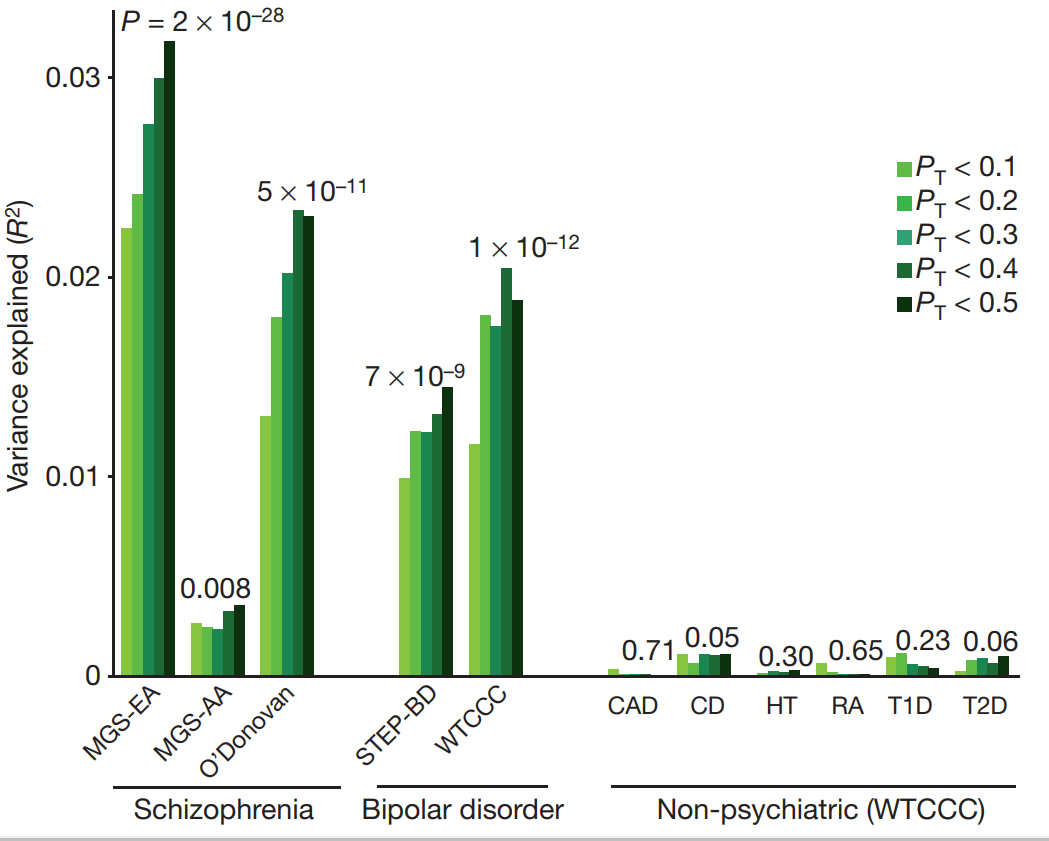
\includegraphics[width=3in]{images/background/prs.png}}
\caption{{\bf Calculated Polygenic component of Schizophrenia and Bipolar disorder, as well as non-psychiatric\cite{Consortium2009}} Calculated $R^2$ for Schizophrenia, Bipolar Disorder using different SNP thresholds. On the right are some common diseases. CAD, coronary artery disease; CD, Crohn’s disease; HT,
hypertension; RA, rheumatoid arthritis; T1D, type I diabetes; T2D, type II
diabetes.}
\label{prs1}
\end{figure}


\subsection{LDPred-funct}
LDPred-Funct by Dr. Marquez-Luna et al\cite{Marquez-Luna375337} is an extension of the LDPred algorithm first described by Vilhjhálmsson et al\cite{ldpreeed}. The LDPred algorithm increases the results obtained in PRS by modeling the Linkage Disequilibrium instead of pruning it (as the P+T method). This is done by estimating the posterior mean effect size of the given markers when fed LD information from an external cohort as well as prior information on those effect sizes. LDPred-funct then builds upon this system by incorporating into the model the trait-specific functional enrichments. Annotations are fit upon these functional priors and afterwards the LDPred-funct estimates the posterior mean effect size using these enrichments and annotations. A Cross-Validation method further improves the stability of the prediction as it does CV within samples, regularizing casual effect sizes.These improvements allow it to outperform the previous methods, as shown in Figure \ref{ldpred1} 

\begin{figure}[!ht]
\centerline{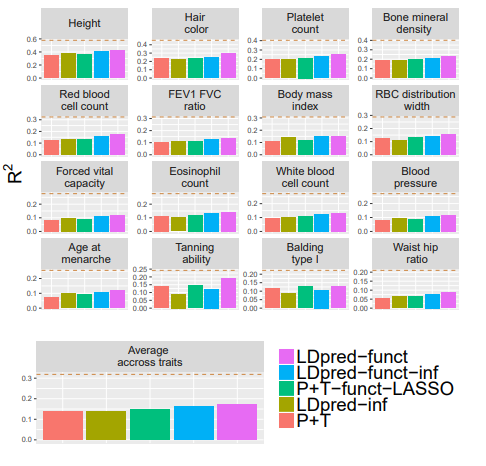
\includegraphics[width=3in,]{images/background/ldpred.png}}
\caption{{\bf Accuracy of PRS prediction methods on different UK BioBank phenotypes\cite{Marquez-Luna375337}} $R^2$ Results using 5 different polygenic methods using the UK BioBank dataset and evaluating 16 different phenotypes. The $R^2$ value is compared against the maximum calculated heritability value at the top of the graphs.}
\label{ldpred1}
\end{figure}
\clearpage
\section{Alzheimer Disease}

In this section the underlying theory behind Alzheimer Disease is explained as well as the progression that occurs from a person who is Cognitively Normal up to the point where Alzheimer Disease develops and Dementia is diagnosed. The multiple factors that are theorized to lead to the disease are also explained.

Alzheimer Disease is a neurodegenerative disease which targets an estimated 24 million people worldwide according to Ballard et al\cite{Ballard2011}. As he describes, the main markers in a person with Alzheimer Disease are formation of amyloid plaques and neurofibrillary tangles. Once a person begins to develop Alzheimer what occurs is that the $\beta$-Amyloid peptide 42 is generated from the amyloid precursor protein which then begins to store in the neuron and outside starts forming the plaques.These plaques then begin to form a cascade of sorts which slowly leads to cognitive impairment in the brain and finally to death. 

Mudher and  Lovestone\cite{Mudher2002} have proven one of the multiple hypothesis regarding the development of Alzheimer: A specific protein called $\beta$-Amyloid starts to develop in the brain, generating an excess formation of $\beta$-Amyloid plaques which in turn start blocking synapses between neurons in the brain and thus the breakdown of neurocognitive capabilities begins in a cascading manner. The Amyloid precursor protein suffers a fault in the onset of Alzheimer, which thus creates an Amyloid peptide A$\beta$1-42.
This peptide is the one that begins creating plaques and creates a cascade of other problems like tau aggregation and neuronal attrition. Figure \ref{gr1} shows the causes and development of plaques and the corresponding Dementia diagnosis.
\label{betaAmyloid}

\begin{figure}[!ht]
\centerline{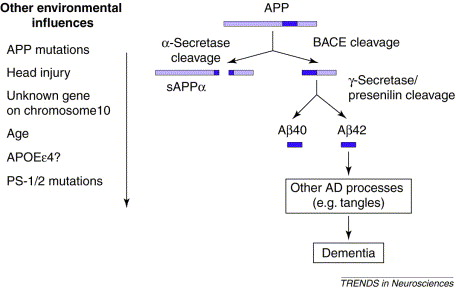
\includegraphics[width=4in]{images/background/gr1.jpg}}
\caption{{\bf Plaque formation and possible causes\cite{Mudher2002}} Development of Alzheimer's disease relating to the procedure via which the APP protein converts into Amyloid plaques that cause the disease. On the left are some possible environmental influences including the APOE $\epsilon4$ gene}
\label{gr1}
\end{figure}


Multiple other hypothesis exist for Alzheimer disease\cite{Scheltens2016} such as the tau hypothesis and retro-genesis. One of the main genetic component associated with the disease is the APOE $\epsilon4$ variant, if present, this variant reduces the breakdown of $\beta$-Amyloid in the body and thus an increase in plaques. The $\beta$-Amyloid hypothesis and its variants has shown in various tests a strong correlation which does indicate the right direction, but there are still multiple areas where research can grow to explain holes in the current formulation.

Meanwhile the Tau protein is the one which causes the aforementioned tangles, This protein is modified via the presence of a high concentration of $\beta$-Amyloid and results in the creation of some insoluble compounds that cause the neurons to cease functioning correctly. The Tau proteins also start forming sheets which are then transmitted to other parts of the brain and result in the spread of the disease. 
\newpage
Scheltens gives \cite{Scheltens2016} some other Biomarkers besides Tau protein concentration and $\beta$-Amyloid plaques to detect Alzheimer. Some of the are A$\beta$ oligomers, some synaptic proteins such as neurograning and SNAP25. These are found in the cerebrospinal fluid and as such are not so easy and cheap to detect. Thus he also mentions some blood biomarkers, one example being CNS proteins, but this area is still lacking.

In the same paper \cite{Scheltens2016} it is shown that the lifestyle and demographics of the patients can affect the risk factors of developing Alzheimer. Clearly the main factor is age, but Diabetes, Obesity, lack of mental stimuli and depression can increase this risk by up to 30 percent.

Ballard demonstrates that not only biomarkers play an important role, but that the genetic code has a high impact on the formation of Alzheimer, as some genes promote the formation of Tau sheets via generation of compounds that phosphorilyze Tau proteins, others increase the burden of  $\beta$-Amyloid particles and some others increase the amount of Amyloid precursor protein available. These genes can increase the risk of Alzheimer by up to 70 percent. Scheltens also agrees on this point and does show the same results regarding the genetic factor.

The Early Onset disease follows a very Mendelian inheritance pattern, with mutations in the APP, PSEN1 and PSEN2 related genes causing the disease almost certainly. But the genetic component of Late-Onset Alzheimer is a much more complex one. As seen before it is one of those multifactorial, complex and polygenic diseases that are most complex to determine. The APOE $\epsilon4$ variant is definitely the main genetic factor to consider as a risk indicator, but multiple other genes have been shown to have correlation with the disease as CLU, ABCA7, BIN1 and others which can be seen in Figure \ref{genAD}. Most of these genes have been shown to have a biochemical relationship with the  $\beta$-Amyloid production process, and as such they are not only statistically significant. There are variants in multiple pathways each of which gives a very small risk increase but can overall have a large impact on the risk factor which is then further amplified by the environmental factors. Furthermore, some mutations have compounding effects, one SNP in PSEN1 with patients who also carry the APOE $\epsilon4$ mutation have a much higher risk of developing the disease than those that don't have both mutations. Thus, approaches that use a multitude of genes with nonlinear combinations might perform better than single-SNP diagnosis.\cite{KARCH201543}

\begin{figure}[!ht]
\centerline{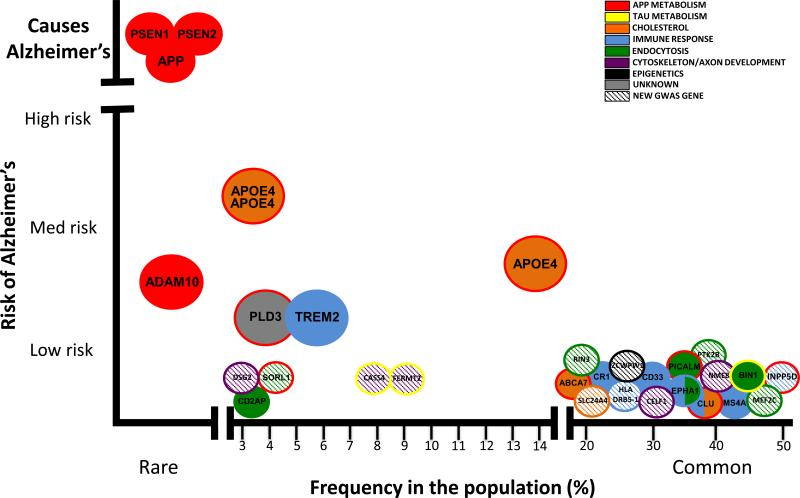
\includegraphics[width=4in]{images/background/genad.jpg}}
\caption{{\bf Genetic variants that contribute to Alzheimer's Disease\cite{KARCH201543}} These are some of the genes as well as the biological functions they play that increase the risk of developing Alzheimer's Disease}
\label{genAD}
\end{figure}


As shown by the National Institute on Aging\cite{McKhann2011}, the clinical diagnostic of Alzheimer's disease (and by proxy, the stages leading to it) is quite complex. The one way to know without a doubt if a patient has Alzheimer's Disease is by doing a postmortem autopsy and finding the amyloid plaques that impair the brain, this is useful for research but clinically speaking it is pointless. Other diagnosis while the patient is alive consider the use of cognitive tests to test the patient's ability to memorize or perform complex tasks. Bio-marker concentrations seen before can also be used to diagnose the state of Alzheimer's disease. Furthermore this problem is complicated as someone who might not have Alzheimer's (Or even any type of Cognitive Impairment) could develop the disease after some years, with very different rates of development across individuals. Some patients go from Cognitively Normal to Alzheimer's almost directly, some never make the jump from Mild Cognitive Impairment to AD, and some others can have a regression (Mostly due to clinical or test errors) Thus, this makes it so that working with Alzheimer's databases for diagnosis something quite complex as there is uncertainty regarding whether the sample being analyzed is truly a control or if it is just a case lying dormant as a control for the point in time taken.

Due to some of the complications present in the clinical diagnosis there is also interest in detecting the presence of Alzheimer's Disease or possible early signs of the development by the use of longitudinal data using Biomarkers or Magnetic Resonance Imaging as an aid to help the detection process. These models could take the data of a given patient and tell the doctor through an analysis why the system believes the patient to have the early signs of Alzheimer's which are consistent with the results found in other patients. By detecting it in an early stage the patient can start taking decisions with respect to the disease and analyze prospective treatments before it is too late.

The gold standard though, would be the prediction of Alzheimer's disease decades before it's onset, or at least a risk indicator which could give the patient the knowledge required to make environmental changes that might slow down the progression of the disease or the use of medicines designed to have an impact at the earliest stages of the (as is the case with most drugs being analyzed that stop the amyloid plaques from developing). 
\clearpage


\section{Machine Learning}

Machine learning is a form of data analysis that has existed for decades but has recently seen a big increase in terms of popularity and performance thanks to the increase in available data as well as processing power. Through the use of a plethora of algorithms and models a computer can be trained to find specific and desired patterns in a sea of data to accomplish reliably a given task such as detecting a disease. Machine learning is commonly split in three categories: Supervised Learning, Unsupervised Learning and Reinforcement Learning. The first category is the one of interest in this thesis, where the algorithms are given sets of labeled data from which to learn and adjust across multiple iterations depending on the correctness of the prediction. Then the resulting model is extrapolated to a validation or testing dataset to ensure the performance is valid.

This section gives the background information of the machine learning methods used in this thesis. It begins with describing Support Vector Machines(SVM), and Random Forest(RF). Afterwards an in-depth description of Neural Networks and Deep learning is given with the multiple hyper-parameters that can be tuned and adjusted. Then it gives an analysis of the FRESA.CAD benchmark as well as the component methods that are used by it.

\subsection{Support Vector Machines}
\label{RF}
Support Vector Machines are Machine Learning models first proposed by Boser, Guyon and Vapnik\cite{Boser:1992:TAO:130385.130401}. SVMs try to optimize the problem by finding a hyper-plane in the feature space being given as input where it can distinctly classify the two different classes. This is obtained by maximizing the margin between the chosen hyper-plane and the so-called Support Vectors. Support Vectors are the sample points close to a given hyper-plane that would then give the location and orientation of the classifier, and which are iterated and selected to obtain different points. Thus, by maximizing the margin finding a boundary in a higher-dimensional space where it can separate the classes apart. Figure \ref{svm1} shows an example of how the SVM Hyper-plane is selected and the role the Support Vectors play in maximizing the margin, as shown the Support Vectors chosen tend to be those close between the classes. This is further expanded upon by using something called the kernel trick, where a transformation is done to the input where it is extended into a higher-dimensional space and depending on the chosen kernel gives a Non-linear representation of the data where the hyper-plane separation can be done. This then allows a more robust and complete transformation allowing non-linear classification. 

\begin{figure}[!ht]
	\centerline{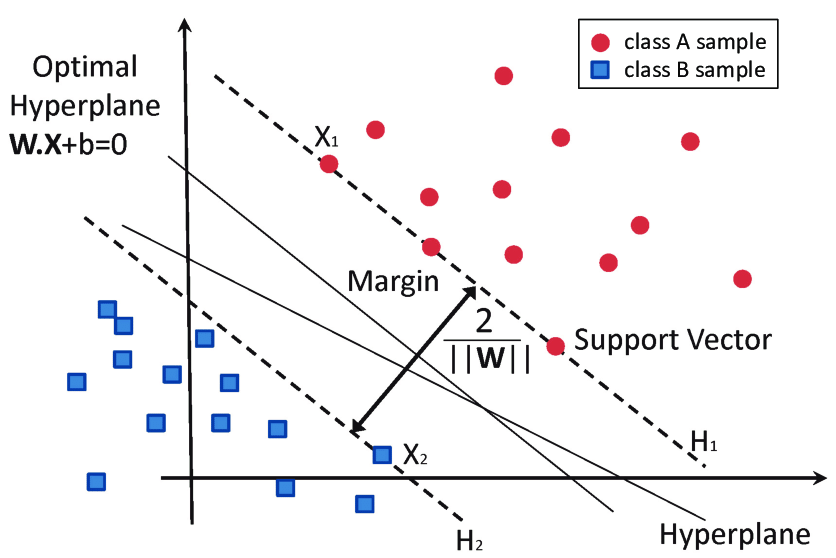
\includegraphics[width=5in]{images/background/svm.png}}
	\caption{{\bf Support Vector Machine Hyper-plane classification \cite{svm1}}
		An example of the hyper-plane classification being done by a SVM. The data samples from different classes nearby are chosen as Support Vectors and a hyper-plane is chosen which maximizes the margin between classes.} 
	\label{svm1}
\end{figure}

\subsection{Random Forest}

Randoms Forest is another Machine Learning method which can be used for the classification task. It was first presented by Ho\cite{598994} and also gives very robust and precise results. It works by doing an ensemble of a multitude of Decision Trees, from which it then takes the mode of the results given by all of trees. Each tree is given a random subset of features from the total input features and then builds the tree using the best features out of that subset.  Thanks to using different decision Trees, each of which uses a different random subset of features for the classification task the random forest helps avoid over-fitting and obtains results that are more accurate and stable on the validation results as a Wisdom of the Crowd model. Figure \ref{rf1} gives an example of the structure a Random Forest follows.

\begin{figure}[!ht]
	\centerline{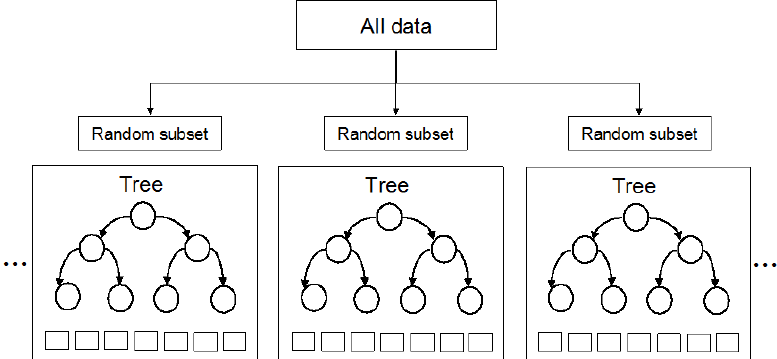
\includegraphics[width=5in]{images/background/rf.png}}
	\caption{{\bf Random Forest Structure\cite{rf}}
		The diagram shows an example of the structure a Random Forest follows, with different trees each using a subset of random features.} 
	\label{rf1}
\end{figure}

\clearpage
\subsection{Neural Networks and Deep Neural Networks}
\label{DNNs}
Artificial Neural Networks (ANN) are yet another Machine Learning tool for supervised learning. The basis of an ANN is the perceptron, dating back to 1958 and first described by Rosenblatt\cite{Rosenblatt58theperceptron:}. This is a mathematical model based on the neurons of the brain, where there are multiple inputs each multiplied by given weights that enter the perceptron, and in some cases applying an operation (Activation Function), which gives an output consisting of a linear combination of these features. Figure \ref{percep1} gives a visual description of the model a perceptron follows. A simple perceptron thus can be used as a classifier, where it will be able to do linear classification and as such is limited. 

\begin{figure}[!ht]
	\centerline{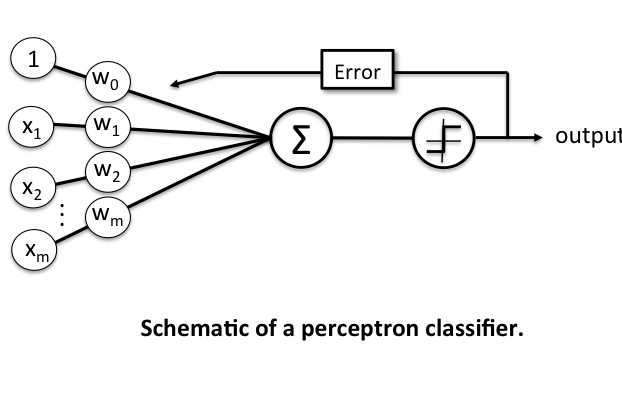
\includegraphics[width=5in]{images/background/perceptron.png}}
	\caption{{\bf Perceptron Model\cite{percep}}
		The model describes a simple single-layer perceptron with the inputs on the left, followed by the weights by which to multiply them, the sum done in them and finally the activation function that leads to the output. The feedback error to guide the learning process is also shown.} 
	\label{percep1}
\end{figure}
When using multiple layers of these perceptrons the performance and prediction capabilities of the resulting network is greatly enhanced. These multi-layer perceptrons (MLP) are thus Artificial Neural Networks, an homage to the biological source of inspiration (Even if the similarity is no longer there). Artificial Neural Networks typically consist of an input layer, which is then connected to an intermediate (or more) hidden layer (named as such as it is not directly observable), the hidden layer then connects to the output layer and gives a result. Then this output is compared to the actual label and the network is adjusted accordingly. A series of iterations are run with the available samples and across multiple repetitions called epochs to successively train the network.

Two methods are crucial to the inner working of the ANNs: Forward-propagation and Backpropagation. The first is the one responsible to propagate the input data across the successive hidden layers until it reaches the output layer. It does this by the previously described method in the perceptron multiple times over both in terms of layers and in terms of the respective neurons per layer. Backpropagation takes the error value obtained when comparing the obtained output with the real output, and obtaining the error derivatives for the output layer, then sending that backwards towards the hidden layers and all the way back. The derivatives are then used to calculate the adjusted values of the weights to correct this error and the model is updated. By using the gradient respective to each weight each of them is adjusted towards the correct direction for a precise result. The weight update incorporates an important value: the Learning rate, this is a hyper-parameter than will control how much the weights will be update iteration, to ensure the learning is not done too slowly, but that it doesn't overshoot either. Figure \ref{dnn1} gives an example of the architecture of a neural Network, while also describing the forward-propagation and the backpropagation methods in a visual manner coupled with the respective mathematical formulation.

\begin{figure}[!ht]
	\centerline{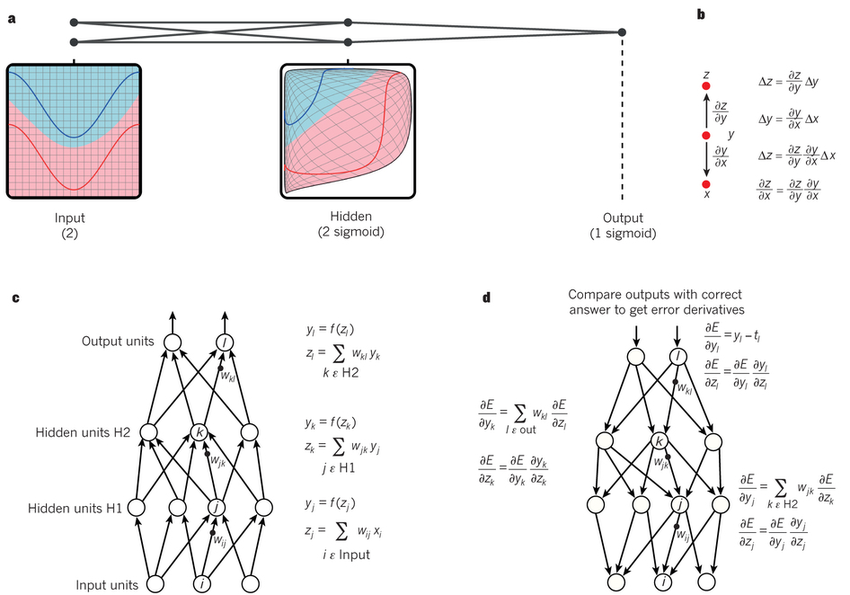
\includegraphics[width=5in]{images/background/deepnet.png}}
	\caption{{\bf Neural Networks, Forward-propagation and Backpropagation\cite{LeCun2015}} a) shows how MLP can make an input linearly separable by transforming the input space. b) shows the backpropagation error equation in terms of derivatives. c) gives the forward-propagation equations in a sample DNN, while d) describes the backpropagation } 
	\label{dnn1}
\end{figure}

According to Yann LeCun\cite{LeCun2015} Deep Learning is a method which allows to learn the representation models of data using multiple processing layers. Thanks to how the model is distributed in multiple layers and each layer affects the next ones the higher-order layers begin to learn more abstract structures in the data which are not detected in the first stages and can thus give a better solution to a given problem. Furthermore the different layers can use back propagation to give feedback to lower layers on which weights to adjust from the neural links and thus improve the representations all across the network. 

Schmidhuber defines\cite{Schmidhuber2015} the description of what makes a neural network deep: it has a considerable depth of its credit assignment paths which tends to be larger than 3. This depth and the choice of how many hidden layers as well as how many neurons will be present in each layer are the most important parameters to modify when creating a deep neural network and can have quite varying degrees of success. 

An activation function is a crucial component of a neural network node. These are the functions that describe how the neural network will interpret the sum of its inputs and thus obtain one output. Multiple activation functions are used and the results of the network can vary greatly depending on them. Some examples of activation functions are: Logistic, Rectified Linear Unit(ReLU) and its variations, Binary Step, TanH, Softplus, Gaussian, etc. The most commonly used activation function is the ReLU, first described by Nair and Hinton\cite{Nair:2010:RLU:3104322.3104425}. This activation function has multiple benefits arising from a more biologically-inspired perspective:

\begin{itemize}
	\item It has no output values other than 0 when having a negative inputs, consistent with biological neurons. 
	\item It propagates the gradient efficiently.
	\item It has a sparse activation, which allows the model to learn more efficiently in a distributed manner. 
	\item it is scale-invariant with respect to the input.
	\item It is computationally efficient thanks to using only addition and multiplication.
\end{itemize}
\newpage
The equation for the ReLu is quite simple and is as follows:

\begin{center}
	$f(x)= max(0,x)$
\end{center}

One of the main problems with Neural Networks which also has a greater impact for Deep Networks is the vanishing gradient problem, as the gradient is sent forward and backwards using the gradient of the chosen error function the gradient starts to get smaller and smaller due to applying the chain rule with functions from -1 to 1.  The ReLU unit can reduce the vanishing gradient problem thanks to how it goes from the desired value to 0 directly when it detects a 0 or lower in its input

The selection of a Loss function for the Neural network is another factor which can be modified to obtain different results. The Loss function indicates how the resulting output is valued and thus how back propagation will be calculated and sent back throughout the whole network. Thus it encodes the cost or value of giving a specific output depending on the real world solution desired. Back propagation calculates the gradient of this loss function and then updates every neuron through it. Multiple loss functions can be used and this will modify the way the neurons will learn and the weights will be modified, thus care must be taken. There are multiple cost functions, some of the most common ones are Mean Squared Error, Root Mean Squared Error, Soft max. For classification problems one of the most widely used is the Cross-Entropy Loss which is described by the following formula given 2 possible classes (where y is the real label and p the predicted label):

\begin{center}
	$-(ylog(p)+(1-y)log(1-p)$
\end{center}

This loss function will try to minimize the distance between the predicted probability distribution and the real probability distribution of the classes. To correctly use Cross-Entropy the output of the final layer must be a probability and as such the final output layer must be a Sigmoid activation function or similar. Additionally, Cross-Entropy improves the Sigmoid activation by avoiding getting the neuron saturated and will not slow down the learning process.

The final choice of crucial hyper-parameter to tune in the Deep Learning Networks is the Optimizer. These are the algorithms responsible to minimize the desired loss function by adjusting the weights, bias and in some cases the learning rate. Typically these use the Gradient of the function as described before to calculate the adjustments (But some can use the Hessian). Some of the classical optimization algorithms for Neural Networks are Gradient Descent with its variants such as Batch and Stochastic Gradient Descent, Momentum Descent, Rmsprop, Adagrad among others. 

But typically one optimization algorithm is used almost always above the others due to its performance in multiple tasks: Adam. Adam is an optimization algorithm developed by Kingma and Ba\cite{DBLP:journals/corr/KingmaB14} which extends the Stochastic Gradient Descent algorithm. Its name stands for Adaptive Moment Estimation, and it does it by adapting the learning rate for each parameter based on estimates of the mean (first moment) and the variance (second moment) of the calculated gradients. Some of the benefits of this algorithm are the following:

\begin{itemize}
	\item Efficient to calculate and cheap to store.
	\item Easy to scale.
	\item Few tuning parameters to adjust.
	\item Works correctly with sparse or noisy datasets.
\end{itemize}


One of the main problems of DNNs (and in Machine Learning in general) is overfitting, where the learned model trains too much on the training set, memorizing it perfectly but while doing this it loses the ability to generalize and performs worse in samples that have not been seen before (such as the validation dataset). This is a deal-breaker for most applications and as such multiple methods have been traditionally used to process the data, reducing the over-fitting and increasing the performance on the validation dataset. Dropout, Normalization and Regularization are the main tools employed to achieve this and most DNN currently use a mixture of them.

Dropout as a method was first proposed by Srivastava, Hintont et al\cite{JMLR:v15:srivastava14a} in 2014 as  a powerful yet simple way to minimize overfitting and thus making the algorithms more precise in the validation and training stage to be able to generalize without specializing too much into the training set. Dropout as a concept is very simple. Neurons are randomly deactivated with a given probability all across the network in the training phase, which means they don’t affect the next layers and they do not learn (Those weights are effectively frozen). This allows to sample a thinned out version of the network, and each of the iterations has a different thinned network, all of these get combined. This can be seen as a way of putting together many different models to get a prediction which in average performs better. Also, the way this is done enables the training to be spread around the different neurons and weights instead of being specifically trained just for one case. Dropout has been so efficient at preventing overfitting that it is the most widely used 


L2 regularization has been used by many researchers, such as Andrew Ng which was one of the first to apply it for Neural Networks\cite{Ng:2004:FSL:1015330.1015435}. Regularization is used to penalize more complex models (which are more prone to overfit the data), by minimizing both the Loss function and the complexity of the model. The L2 equation is the sum of the squares of all weights at a given layer, and it is expected to be as low as possible. L2 regularization will then penalize harshly those weights that have a strong impact with respect to the other weights and will try to keep them close to zero, thus reducing the complexity of the model and regulating the weights across the layer. This will most certainly decrease the overfitting while maintaining good performance.

Batch Normalization is a method created by Ioffe and Szegedy\cite{Ioffe2015BatchNA}, used in tandem with Batch updating which normalizes the activations across the batch. It analyzes the mean and variance present for every feature in the training batch and then normalizes the inputs by subtracting the mean and dividing by the standard deviation, then scales and shifts the normalized activations. Batch normalization helps control the magnitude of the activations and as such smooths the loss function (as well as damping oscillations) which makes the corresponding optimization process work in a more efficient way. 


\subsection{FRESA.CAD Benchmark}
\label{fresaCAD}
FRESA.CAD is a benchmarking package in R ( openly available in the CRAN) created by Dr. Taméz Peña\cite{fresa}, which evaluates the repeated holdout cross-validation (RHCV) of binary classification algorithms or feature selection (FS) algorithms, and returns a set of all the test results. Figure \ref{fresafig1} shows the RHCV implemented in FRESA.CAD. The repeated test results are then combined into a single prediction per sample, returning the classifier performance for further analysis. The summary performance statistics also include the 95\% confidence intervals to check statistical confidence. The implemented RHCV also returns the selected features at each train instance. 

\begin{figure}[!ht]
	\centerline{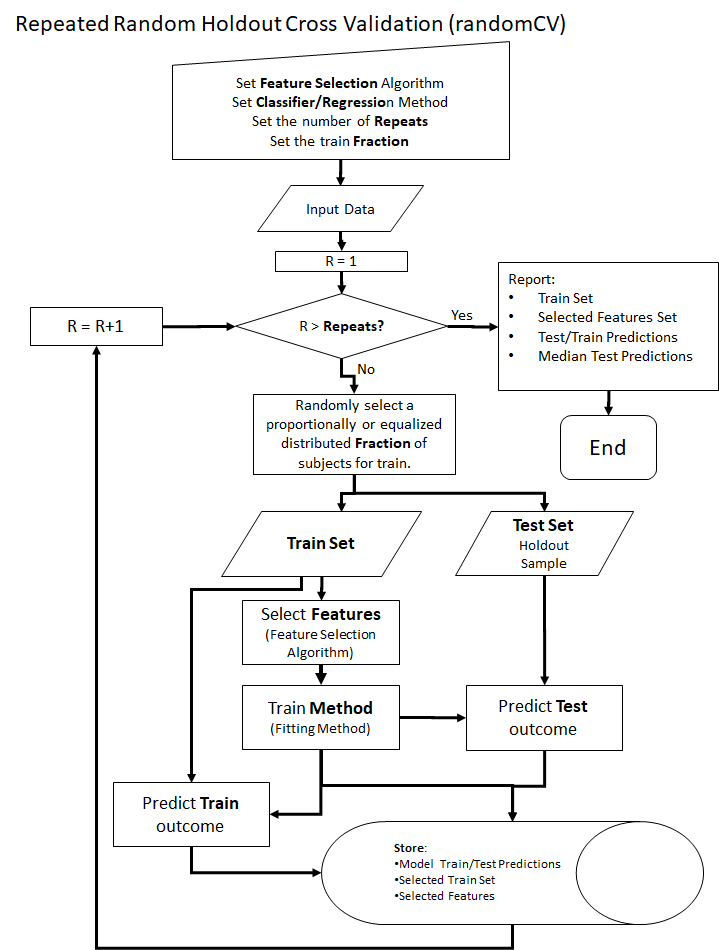
\includegraphics[width=4in]{images/background/fresaRCV.png}}
	\caption{{\bf Repeated Holdout Cross-Validation with FRESA.CAD\cite{fresa}}
		The flow diagram depicts the RHCV procedure implemented in the FRESA.CAD benchmark used to split the input dataset for training and validation} 
	\label{fresafig1}
\end{figure}


All of these factors make it so that there can exist a comparison between different classifiers and feature selection algorithms under the same environment, ensuring there is no variation due to train/test sets or filtering algorithms. The benchmark takes a dataset and runs a set of predetermined classifiers and feature selection algorithms. Furthermore, FRESA.CAD allows the simple exploration and comparison of the selected features of each filter method to identify features that could be of use. Figure \ref{fresafig2} shows the workflow of the benchmark procedure, which by default uses Bootstrap Stage-Wise Model Selection (BSWiMS) as the data-classifier method.

\begin{figure}[!ht]
	\centerline{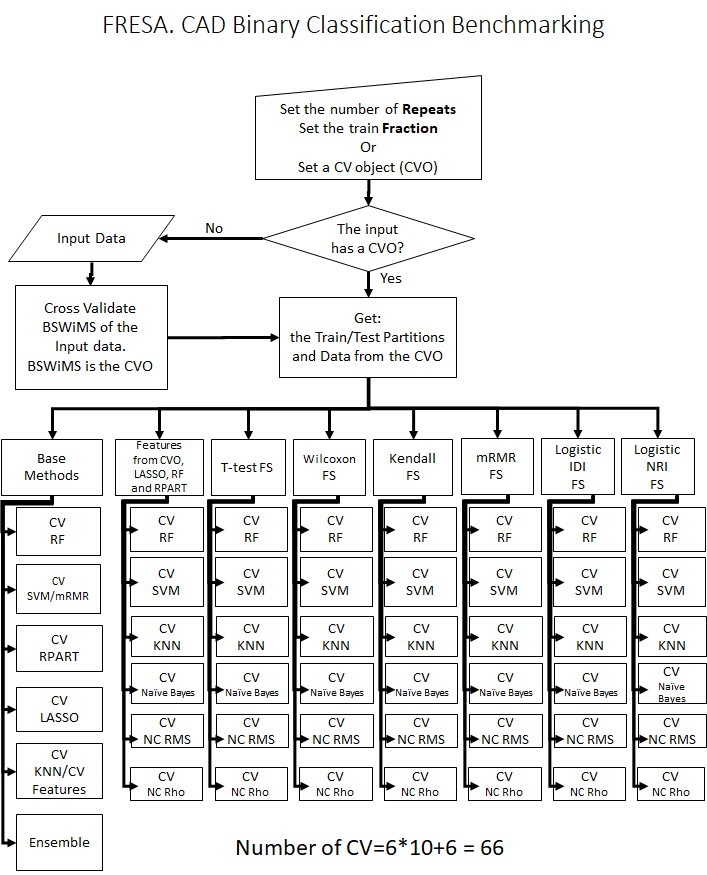
\includegraphics[width=4in]{images/background/FresaBinBen.png}}
	\caption{{\bf FRESA.CAD Benchmark procedure\cite{fresa}} The flow diagram depicts the Benchmarking procedure across the different models and filters for comparison in each Cross-Validation iteration}
	\label{fresafig2}
\end{figure}

The results of the Cross Validation instances executed by the FRESA.CAD Binary Benchmark can be compared with the performance statistics and they are then ranked by comparing each CV instance 95\%CI. The ranking method accumulates a positive score each time the lower CI of a performance metric is superior to the mean of the other methods and loses a point each time the mean is inferior to the top 95\%CI of the other methods. Additionally, the package returns the accuracy, precision, sensitivity, the balanced error rate and the ROC area under the curve with their corresponding 95\% confidence intervals (95\%CI). The plotting functions included with the package make the visualization and comparison much easier and useful.

\clearpage

\section{Previous Work}

The first segment will describe work done with Deep Learning using genetic data with different diseases. Another topic described will be the detection of Alzheimer disease via Machine Learning methods to give an overview of what has been done and has worked to detect it directly based on observations, Finally, the state-of-the-art as well as investigations previously taken in the area of Alzheimer Disease prediction are described.
 
\subsection{Genetic Prediction with Deep Learning}

Deep Learning has recently arisen as a tool used for Genomics analysis to understand the vast amount of data available in all the different pathways of the chromosome. Thanks to the processing power of Deep Learning the vast number of links and relationship among genotypes, phenotypes, proteins, regulation and others could be understood with more precision. Deep Learning must be implemented with care and following appropriate guidelines to ensure the models do not overfit or the results given are not biologically consistent.\cite{Zou2019}

One such use of Deep Learning is by Sundaram et al\cite{Sundaram2018}. They describe a method via which they can predict the clinical impact of human mutations, selecting those variants that actually do have an impact in terms of diseases instead of those variants that are harmless. They start from the idea that those mutations that are present across multiple other species will also be benign for humans, thus reducing greatly the number of SNPs to look for disease correlation. They train a deep neural network on the primate and human datasets which learns to predict the pathogenicity a mutation will have based on the change in amino-acid sequence . This is supported by two other networks that predict the secondary structure and the solvent accessibility of a given amino acid sequence. Figure \ref{predHum1} shows the general structure of the algorithm used as well as the results obtained, of note is how the Deep Network correctly assumes that mutations in the functional domains give a higher risk score. This method then identifies rare diseases and the respective genes that cause them with 88\% accuracy, while also giving 14 possible new candidate genes that are related to intellectual disabilities. Thus showing the value of Deep Learning applied to a genomics problem.

\begin{figure}[!ht]
\centerline{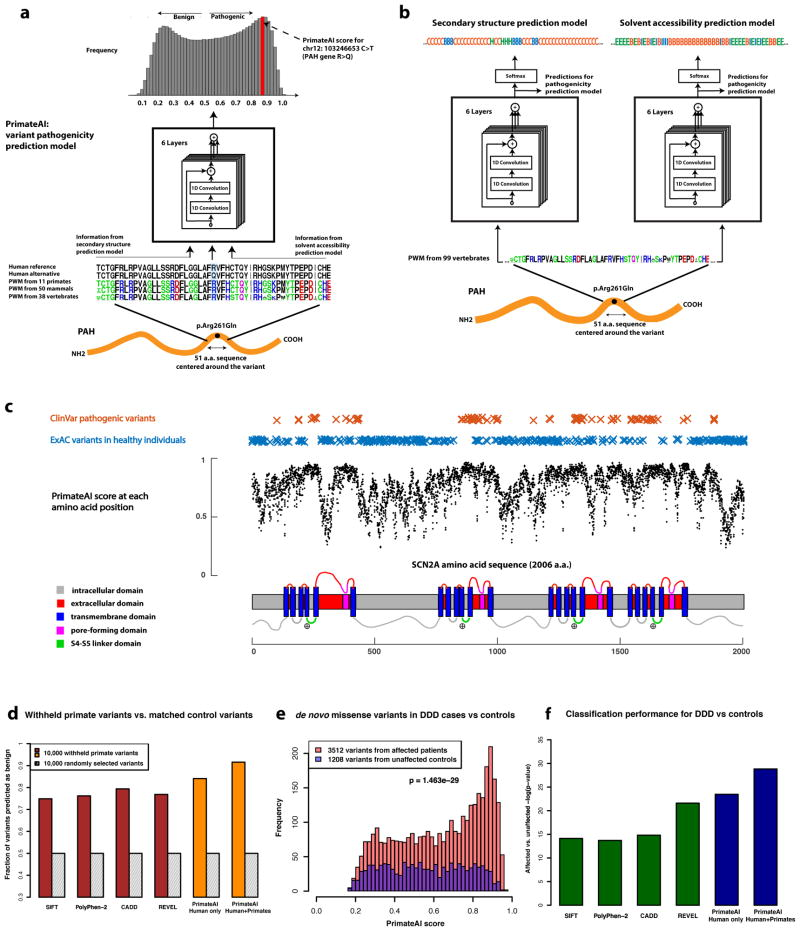
\includegraphics[width=5in]{images/background/predHum.jpg}}
\caption{{\bf Deep learning Architecture and results\cite{Sundaram2018}} Image a) describes the deep network architecture to predict pathogenicity depending on the given Amino Acid sequence variant, the reference and the support network results. Image b) describes the structure of the support deep networks for predicting the secondary structure and the solvent accesibility. Image c) shows the predicted pathogenicity given to mutations at specific points, as well as the reported ClinVar pathogenicity.  Image d) e) and f) give the results obtain with respect to withheld variants, missense variants and classification performance}
\label{predHum1}
\end{figure}
\newpage
\clearpage
Another approach using Deep learning is from Zhou and Troyanskaya\cite{Zhou2017}. They designed a method by which they can predict the effect that de-novo noncoding variants can have. Traditionally, the noncoding variants are ignored with respect to coding SNPs, but using the Deep-Convolutional-Based DeepSEA framework the model can use the data from noncoding variants to predict the impact they will have. The structure followed can be seen in \ref{predeff1}.

\begin{figure}[!ht]
\centerline{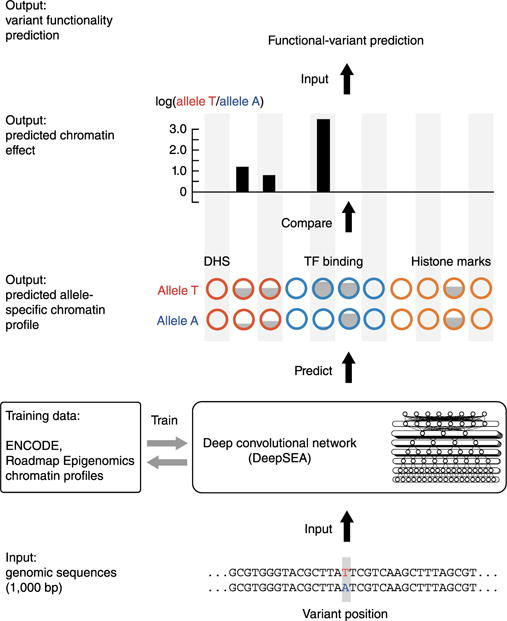
\includegraphics[width=4in]{images/background/predeff.jpg}}
\caption{{\bf Overview of the prediction Architecture\cite{Zhou2017}} The diagram describes the schematic overview of the system. The Deep network receives the sequence at the genetic variant, from which it predicts chromatin profiles contrasts it between the reference and the variant and thus obtains a prediction on the functional effects.}
\label{predeff1}
\end{figure}
\newpage
\subsection{Alzheimer Disease Detection}

Machine Learning approaches for Alzheimer detection have seen a surge in interest in the latest decade. Mishra et al introduce\cite{Mishra2017} a method via which they use the AV-1451 PET Imaging to obtain readings of tau particles which they then parse using unsupervised learning the results of the imaging to find the most informative segments of the brain. Orrú et al show\cite{Orru2012} a Support Vector Machine approach to identify and detect useful biomarkers for prediction and detection of Alzheimer Disease as well as other mental diseases Klöppel et al\cite{Kloppel2008} also use the Support Vector Machine model to classify Alzheimer Disease from a group of patients using MRI scans and achieving up to $96\%$ accuracy.


Neural Networks are an ideal approach for Alzheimer Detection as the causes of the disease are still not very well understood and a myriad of factors can increase the chances of someone developing it, with most of them working in tandem or affecting each other. Multiple biomarkers, genetic information, demographics and even lifestyle habits can be used as input features together. A neural network can take all of these features, understanding and estimating the inherent underlying nonlinear models. This allows it to construct, thanks to its intrinsic learning of representation models, a good estimator of the way these features interact with each other and signify the onset of Alzheimer, thus detecting it.

One of the approaches for Alzheimer Detection is from Sankari\cite{SANKARI2011165} where they use a probabilistic Neural Network to classify between Cognitive Normal and Alzheimer in a control group. The model uses features obtained from coherence studies from and Electroencephalogram. Using the extracted features from the studies they trained a the probabilistic neural network, containing 4 layers: Input, Pattern,Sum, and Output. By representing patterns using Parzen windows and a Gaussian distribution as groundwork the team was able to obtain up to $100\%$ accuracy in the classification via conventional coherence.

Suk, Lee and Shen\cite{Suk2014} propose a feature representation model for Alzheimer Disease detection which can be used in deep learning. They start with MRI and PET imaging information which they then convert into a high-level latent representation model which contains the shared features rich with information. They utilize a Deep Boltzmann Machine to obtain these feature representations, as it can be seen in Figure \ref{gr2}. With this method they managed to obtain up to $95\%$ accuracy with the ADNI data set in predicting whether a patient would have Alzheimer or not using only the imaging information transformed. The deep networks were capable of extracting the high level patterns and models existing between the data.

\begin{figure}[th]
\centerline{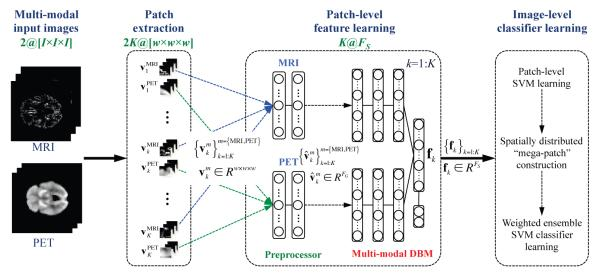
\includegraphics[width=5in,height=3in]{images/background/gr2.jpg}}
\caption{{\bf Suk et al proposed method for deep learning\cite{Suk2014}}{ Method via which they create a feature representation model using deep learning by extracting patches from MRI and PET images which they process and then feed into a Deep Boltzmann Machine, the outputs of which are then classified using a SVM. }}
\label{gr2}
\end{figure}

Liu et al describe\cite{Liu2015} a multimodal approach which tries to solve the problem in efficiency of biomarker representation by using a deep learning architecture. They use the ADNI data set and from those obtained the MRI, demographics, PET data and then assembled them using a Multi-Modal deep network which obtains the fused data representation, this structure can be seen in Figure \ref{gr3}. Then they use this resulting data representation in the network to finally obtain the resulting diagnostic of the disease. The results obtained using this method obtained the best results out of comparisons with Support Vector Machines and gave the best results when they were fused with the most amount of features.

\begin{figure}[th]
\centerline{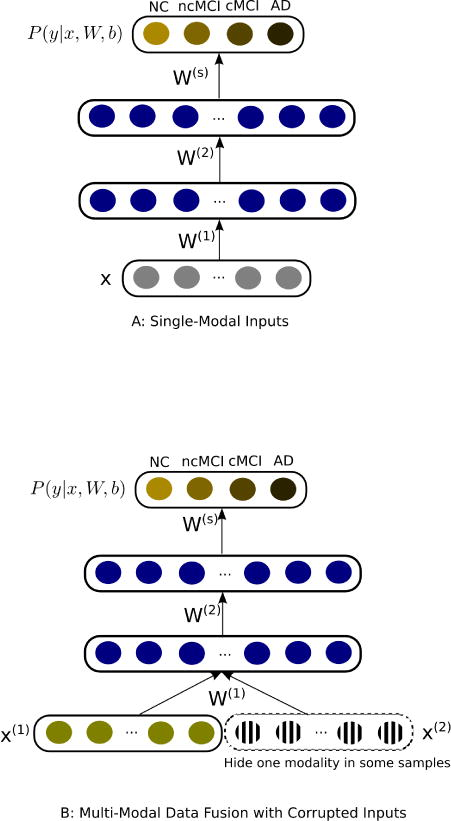
\includegraphics{images/background/gr3.jpg}}
\caption{{\bf Architectures from Liu et al\cite{Liu2015}}{ The architecture used to train Deep Learning architectures, first being single-modal and afterwards with the better multi-modal structure to predict the 4 classes.}}
\label{gr3}
\end{figure}

By utilizing their system they were able to obtain a feature representation in one go while requiring less information and achieving a performance gain.
\newpage
\subsection{Alzheimer Prediction}

The other main component to tackle the Alzheimer Disease problem is prediction. Many proposed medications and treatments are counting on treating the patients before Alzheimer is diagnosed as it is usually too late to have an effect. Thus models that can accurately predict the future development of Alzheimer disease are quite useful for preventive treatments.

Rowe et al created\cite{Rowe2013} an algorithm that could analyze $\beta$-Amyloid imaging, memory performance, hippocampal atrophy and the APOE $\epsilon4$ gene to predict Alzheimer disease after 3 years of the study. By using multivariate analysis they were able to find strong correlations between $\beta$-Amyloid plaques, decrease in Episodic Memory tests and the development of Alzheimer in a couple of years.They were also able to identify that those individuals with high impairment in the EM test and positive $\beta$-Amyloid plaques will progress to Alzheimer. They conclude that $\beta$-Amyloid imaging is a strong predictor of Alzheimer disease.

Mathotaarachchi et al developed\cite{Mathotaarachchi2017a}an algorithm which can assess and predict the development of Alzheimer Disease in a period of two years. They obtain information from the ADNI database using the PET scan regarding the concentration of amyloid particles and then use this information in a probabilistic approach to train a Random Forest-based algorithm called RUSFR (Random under Sampled Forest With this they can then generate predictions in this 2 year interval. Using this method they predicted the results and obtained an area under the ROC curve of 0.906 which performed better than a SVM and L2 Regression. This shows the potential use of only PET imaging data for predicting Alzheimer Disease before its onset.

Long, Chen, Jiang and Zhang describe\cite{Long2017} a method where they utilize MRI imaging to obtain information regarding deformation of the areas of the brain. They then use this data to diagnose and predict the onset of Alzheimer disease. They start by obtaining the distance between subject, and then using a distance matrix and a multi-dimensional scaling algorithm to embed data. This data is then used to classify it via a Support Vector Machine to obtain the resulting diagnosis of the patient. The resulting method correctly differentiated cognitively normal and Mild Cognitive impairment in $96\%$ of the cases and obtained an area under the ROC curve of 0.98 for some specific areas of the brain.
